\iffalse \bibliography{include/backmatter/magnus,include/backmatter/philip} \fi

\chapter{Related Work} \label{section:relatedwork} 
In this section we introduce (i) the process of identifying related work and (ii) discuss state-of-art on the scope of this study. 
%This section aims to justify the need for this study and demonstrate current research. % for the purpose of 
%This section aims to explore literature on using lightweight containers for deployment. 
% aims to show how this research fits into a larger research context 

%-----------------------%
%-----------------------%
%-----------------------%
\begin{table}[ht]
\renewcommand{\arraystretch}{1.4}
\centering
\caption{Start Set}
\label{lr-startset}
\begin{tabular}{| >{\centering}m{1.3cm} |>{\arraybackslash}m{12.7cm}|}
\hline
\textbf{Paper No.} & \textbf{Citation}\\ \hline
\cite{p1}  & C. N. Mao, M. H. Huang, S. Padhy, S. T. Wang, W. C. Chung, Y. C. Chung, and C. H. Hsu, “Minimizing latency of real-time container cloud for software radio access networks,” in 2015 IEEE 7th International Conference on Cloud Computing Technology and Science (CloudCom), Nov 2015, pp. 611–616.                                  \\
\cite{2iot}  & A. Krylovskiy, “Internet of things gateways meet linux containers: Performance evaluation and discussion,” in Internet of Things (WF-IoT), 2015 IEEE 2nd World Forum on, Dec 2015, pp. 222–227.                                                                                                                                      \\
\cite{p3} & M. Raho, A. Spyridakis, M. Paolino, and D. Raho, “Kvm, xen and docker: A performance analysis for arm based nfv and cloud computing,” in Information,Electronic and Electrical Engineering (AIEEE), 2015 IEEE 3rd Workshop onAdvances in, Nov 2015, pp. 1–8.                                                                         \\
\cite{p4} & R. Morabito, J. Kj\"allman, and M. Komu, “Hypervisors vs. lightweight virtualization: A performance comparison,” in Proceedings of the 2015 IEEE Interational Conference on Cloud Engineering, ser. IP10E ’15. Washington, DC, USA: IEEE Computer Society, 2015, pp. 386–393.                                                      \\
\cite{p5} & M. G. Xavier, I. C. D. Oliveira, F. D. Rossi, R. D. D. Passos, K. J. Matteussi, and C. A. F. D. Rose, “A performance isolation analysis of disk-intensive workoads on container-based clouds,” in 2015 23rd Euromicro International Conference on Parallel, Distributed, and Network-Based Processing, March 2015, pp. 253–260. \\
\cite{p6}  & W. Felter, A. Ferreira, R. Rajamony, and J. Rubio, “An updated performance comparison of virtual machines and linux containers,” in Performance Analysis of Systems and Software (ISPASS), 2015 IEEE International Symposium on, March 2015, pp. 171–172.                                                                            \\
\cite{p7} & C. Ruiz, E. Jeanvoine, and L. Nussbaum, “Performance evaluation of containers for hpc,” in Euro-Par 2015: Parallel Processing Workshops: Euro-Par 2015 International Workshops, Vienna, Austria, August 24-25, 2015, Revised Selected Papers. Cham: Springer International Publishing, 2015, pp. 813–824. \\
\cite{p8} & R. Wu, Y. Chen, E. Blasch, B. Liu, G. Chen, and D. Shen, “A container-based elastic cloud architecture for real-time full-motion video (fmv) target tracking,” in 2014 IEEE Applied Imagery Pattern Recognition Workshop (AIPR), Oct 2014, pp. 1–8. \\ \hline
\end{tabular}
\end{table}


\section{Methodology}
The snowballing search approach for systematic literature studies is used to find relevant literature on the topic of this paper. The snowballing search approach is used in order to perform a systematic approach to finding related work. The snowballing approach is complementary to a traditional database search. Specifically, the reference list and citations of a paper are studied in order to identify additional papers that are relevant to this particular review. The snowballing search approach is used to ensure good coverage of current literature in a systematic way.\\

The guidelines for conducting a snowballing search approach, presented by Wohlin \cite{Wohlin} are followed for the search procedure. The steps to conduct a snowballing procedure, depicted in figure~\ref{snow}, involve (i) selecting a set of papers referred to as the start set, (ii) apply forward snowballing and (iii) apply backward snowballing on each paper identified in the set respectively. This process iterates until no new papers are found. To identify a start set of papers, keywords are extracted from the research questions, taking synonyms into account. Formulating a search-string from keywords that are broad and cover multiple areas of research may result in collecting large amounts of literature that span different subject domains. For that reason, broad keywords should be broken down into more specific and detailed keywords specific to the study. The search string is then applied to a database that preferably searches multiple publishers in order to avoid publisher bias. The papers resulting from the database search are then screened and included based on an inclusion and exclusion criteria. An exclusion criteria could state that all online material be excluded. \\

\begin{figure}[ht]
\centering
     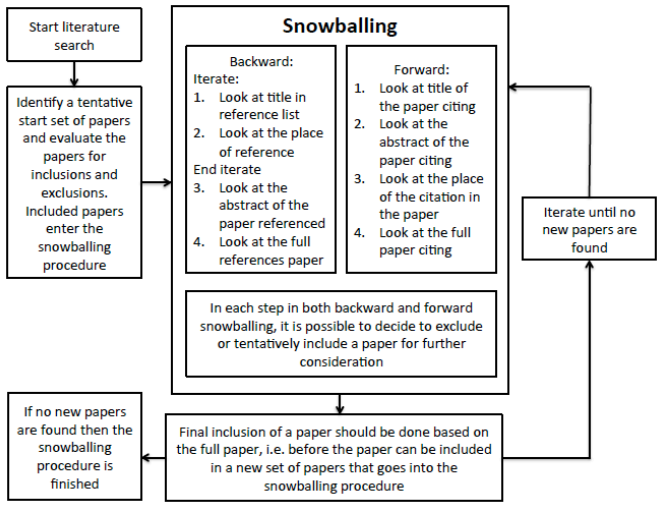
\includegraphics[width=0.8\textwidth]{./figure/snowballing.png}
      \caption{Snowballing procedure \cite{Wohlin}.}
       \label{snow}
\end{figure}

Backward and forward snowballing is then conducted on the start set. Backward snowballing is the process of studying the reference list to identify new papers. Looking at the place of reference and reading the title and abstract of the paper is a good starting point for inclusion, however, final inclusion states that the entire paper must be read \cite{Wohlin}. Subsequently, forward snowballing is the process of identifying papers that cite the paper under inspection. The same process of reading the title, abstract and place of reference is applied in order to include new literature that is found during the procedure. \\

\section{Results}
To gather a start set of papers, a database search on Scopus \cite{scopus} is performed to identify papers from multiple publishers: the precise search string, in the required syntax for Scopus is: \\

{\centering{\small{\textit{TITLE-ABS-KEY(Performance OR Comparison OR Latency OR Evaluation OR Container-Based OR Linux Containers OR Lightweight Virtualization OR Container Cloud OR Docker) AND (LIMIT-TO(SUBJAREA,"COMP")}}}}\\

The search string is targeted at papers identifying the performance cost of using Docker. Applying the search string to the Scopus search function resulted in finding 215 papers from different publishers where no limitation to the search in respect to publication year is made. A screening process is then applied to the 215 papers, reading the title and abstract to see if the paper is related to this study. Papers from the set of 215 is then added to the start set upon meeting the inclusion and exclusion criteria. Papers were included if the data collected in the study is quantitative performance benchmarking. Papers were excluded if being reference to online material or in a foreign language.\\

In total, eight candidates for inclusion were identified. The entire paper for each of the eight candidates is read as a requirement for final inclusion. The eight papers are listed in table~\ref{lr-startset}, in order of reference. Backward snowballing is then applied to all papers in the start set. \textbf{P1} includes 26 references where one reference is already included in the start set (paper \cite{p6}). Based on passing the inclusion and exclusion criteria, one paper is read and passes for final inclusion. The paper identified and thus included is:\\
%-------------------------------
\begin{itemize}
\item \cite{p9} M. G. Xavier, M. V. Neves, F. D. Rossi, T. C. Ferreto, T. Lange and C. A. F. De Rose, “Performance Evaluation of Container-Based Virtualization for High Performance Computing Environments,“ 2013 21st Euromicro International Conference on Parallel, Distributed, and Network-Based Processing, Belfast, 2013, pp. 233-240.\\
\end{itemize}
%-------------------------------
\begin{table}[H]
\caption{Results from Backward Snowballing in Iteration 1}
\begin{tabular}{|>{\centering\bfseries}m{1in} |>{\centering}m{1in}| >{\centering}m{1in} |>{\centering\arraybackslash}m{1in}|}
\hline
\textbf{Start Set Paper} & \textbf{No. References} & \textbf{Reference to Start Set} & \textbf{New Papers Identified} \\ \hline
\cite{p1}              & 26                      & \cite{p6}                                          & \cite{p9}           \\ \hline
\cite{2iot}              & 21                      & \cite{p6}, \cite{p4}                               & 0                   \\ \hline
\cite{p3}              & 47                      & \cite{p6}, \cite{p9}                               & 0                   \\ \hline
\cite{p4}              & 42                      & \cite{p6}, \cite{2iot}, \cite{p9}                    & 0                   \\ \hline
\cite{p5}              & 46                      & \cite{p9}                                          & 0                   \\ \hline
\cite{p6}              & 50                      & \cite{p9}                                          & 0                   \\ \hline
\cite{p7}              & 19                      & \cite{p6}, \cite{p9}                               & 0                   \\ \hline
\cite{p8}              & 18                      & 			                                          & 0                   \\ \hline
\end{tabular}
\centering
\label{back-snow}
\end{table}
%-------------------------------
Table~\ref{back-snow} lists the result of backward snowballing on the remaining seven papers. The results are presented in a table to avoid redundant text as the process and results of backward snowballing for each paper is very similar. In all papers, except \cite{p1}, no new papers matched the inclusion criteria after reading the title and abstract respectively. Furthermore, most of the papers in the start set reference to each other, as seen in column three of table~\ref{back-snow}. All papers in the start set contain reference to \cite{p9}, except papers \cite{2iot} and \cite{p8}. Similarly, all papers in the start set reference to \cite{p6} except papers \cite{p5}, \cite{p6} and \cite{p8}.\\
%-------------------------------

Forward Snowballing is then applied to the papers in the start set. This step involves examining the citations towards all papers that are in the start set. All papers were searched for citations using Google Scholar. The Scopus database was chosen not to be used for the forward snowballing procedure since it was shown that Google Scholar was able to find more papers. Many of the papers in the start have been published recently, which may indicate the lack of citations for some of the papers. During the forward snowballing search, a relevant paper was found in regards to this study. It was then decided to include the paper as part of the related work upon passing the inclusion and exclusion criteria. The specific paper included is: \\

\begin{itemize}
\item \cite{p10} Welch, James Matthew. Performance Optimization of Linux Networking for Latency-Sensitive Virtual Systems. Diss. ARIZONA STATE UNIVERSITY, 2015.\\
\end{itemize}

\begin{table}[H]
\caption{Results from Forward Snowballing in Iteration 1}
\label{forward-snow}
\begin{tabular}{|>{\centering\bfseries}m{1in} |>{\centering}m{1in}|>{\centering\arraybackslash}m{1.8in}|}
\hline
\textbf{Start Set Paper} & \textbf{No. Citations}  & \textbf{New Papers Identified} \\ \hline
\cite{p1}              & 0                       & 0                             \\ \hline
\cite{2iot}              & 0                       & 0                             \\ \hline
\cite{p3}              & 0                       & 0                             \\ \hline
\cite{p4}              & 8                       & \cite{p10}				            \\ \hline
\cite{p5}              & 2                       & 0                             \\ \hline
\cite{p6}              & 81                      & 0                             \\ \hline
\cite{p7}              & 4                       & 0                             \\ \hline
\cite{p8}              & 1                       & 0                             \\ \hline
\end{tabular}
\centering
\end{table}

A second round of backwards and forwards snowballing is applied, as two additional papers to the start set were found in the first iteration.\cite{p9} has 32 references. From the 32 references, 16 references is excluded based on being references to online material. A large number of the resulting references have already been analysed in the previous iteration and no new papers were identified for inclusion. \cite{p10} has 69 references with reference to \cite{p9}, \cite{p4}, \cite{p6}. No additional candidates for inclusion were found when studying the reference list of the paper. A second round of forward snowballing is done. \cite{p9} has been cited by 104 papers. When reviewing the list of cited papers, many of them have already been reviewed during the snowballing procedure.  Analysing the list of papers resulted in no additional candidates for inclusion. \cite{p10} has no citations. This is expected since \cite{p10} is not a published paper. \\

In total, ten papers is included for final inclusion for related work. Two additional papers are included but were not found during the snowballing procedure. The papers were found during the initial phase of the research project. One of the papers not have been found during the database search is a paper authored by C. Berger, which has been accepted for publication but has yet to be formally published. The second additional paper was found during the early stages of the research project and is relevant to this study. The search string includes the keywords present in the respective paper, however it was not found in the search. Since it is relevant to the study, it is included. \\

%  papers captured by snowballing and we still want to include, we should state that together with a justification. That is because, technically, either our snowballing is not very accurate or the paper we want to include is not relevant to this work
%in total the papers bla bla

C. Berger \cite{cberger} presents the exploration of a deployment strategy in the context of self-driving vehicles that utilises lightweight Docker containers. The deployment strategy makes use of a number of Docker containers that build and ship signed packages in a container ready for use. However, the paper does not look to identify the precise performance overhead when using Docker as part of the deployment strategy but addresses the need for it in future work. The deployment of software in \cite{cberger} exemplifies a possible deployment pipeline for resource constrained CPSs, that can be used as inspiration when investigating software deployment by using Docker.\\

The authors of \cite{2iot} identify the challenge of deploying, maintaining and configuring software for IoT gateways and investigate using virtual containers to solve these challenges. The authors identify the performance overhead of using Docker as a deployment platform on two different versions of the Raspberry Pi System on Chip (SoC) computer \cite{raspberry}. They identify that there are clear benefits containerizing applications for deployment on resource constrained devices and further identify the need for such research is the field for IoT applications. This shows there exists a need for continuous deployment for embedded, resource contained and high performing applications. The authors of \cite{2iot} recommend a case-by-case analysis when considering using Docker as a deployment platform for IoT devices. The case-by-case analysis is important as in \cite{gonz} the study also experiment with Docker on a Raspberry Pi SoC computer but do not report any substantial degradation in performance. Further use of Docker as a deployment platform is exemplified in \cite{gonz}. The authors of \cite{gonz} explore using Docker as a deployment platform for a generic modular architecture for industrial automated cyber physical systems. A use case of the modular architecture is applied to the development of an automated guided vehicular CPS. The authors state that having a modular architecture, in the form of Docker containers, decouples the complexity of CPSs into simpler subsystems, that different teams can individually develop on. Development teams can work individually on separate subsystems and utilise Dockerhub, the team collaboration feature built into Docker. The authors of \cite{gonz} conclude that using a real-time enabled Linux kernel is needed for further development of the architecture. There were only two papers found using the real-time enabled kernel when benchmarking Docker performance overhead. This study, through the controlled experiment, aims to provide measurement data when using a real-time enabled OS, fulfilling this gap. \\

In \cite{p6} the paper investigates the performance overhead of using virtual machines, Docker and compares the performance to native execution in the context of cloud computing. To analyse the processing overhead of using Docker, a lossless data compressions utility is used in various execution environments. The authors conclude containers have almost no overhead and recommend a case-by-case analysis as using network address translation and the AUFS storage driver are the only two factors that introduce considerable overhead. However, these factors are likely to become improved in the future. \\

In a study presented by Mao et. al \cite{p1}, the authors investigate the next generation of Radio Access Networks (RANs) used by Telecom providers. Traditional RANs are moving towards software as a service in the cloud \cite{p1} due to being hardware dependent equipment which are expensive and lack scalability. Moving traditional RANs to the cloud as software RANs is a challenging task due to the latency requirements of cellular networks: a similar challenge for software with high hardware dependability and time-sensitivity face the domain of autonomous vehicles. To overcome the time-sensitive requirements of software RANs, the authors use a real-time enabled Linux kernel, specifically the RT\_preempt patch, and measure computational and networking latency when using Docker for real-time applications. The cyclic test \cite{cycl} is used to measure computational latency and is a common tool to measure real-time capabilities of an operating system. However, the cyclic test is not comparable to a CPS as it lacks a supportive middleware. The worst case execution time in \cite{p1} is measured and reported in the study. The results of the study show that running real-time applications inside a Docker container achieves near-native performance, while the performance of virtual machines incur much higher latencies \cite{p1}. However, running multiple Docker containers on different hosts incur higher overhead \cite{p1}. Since CPSs may involve multiple computing nodes, measuring the performance of Docker on multiple hosts for real-time computations requires investigation if considering Docker as a deployment platform for multiple computing nodes.  \\

In a study presented by Welch \cite{p10}, the author identifies the performance overhead of using Docker for latency sensitive applications in the context of cloud computing. In \cite{p10}, the RT\_preempt kernel patch for Linux Kernel 3.18.20 is used to identify the networking performance of Docker containers in comparison to virtual machines. The results show that the Docker containers have generally higher bandwidth and lower latency than virtual machines. However, in both \cite{p10} and \cite{p6} the Network Address Translation (NAT) protocol introduces considerable overhead. NAT is needed when mapping a network to a single internet protocol (IP) address. Further research on this topic is required if the requirements for a CPS require independent IP address for multiple containers. \\

In papers \cite{p6,p10,p3,p4,p7,p9}, chosen not to be further detailed due to their respective execution environments, state that the overhead by using Docker is negligible and CPU, memory, disk and network performance is near native. This confirms that Docker can be used for CPSs but further evidence is needed. However, \cite{p5} presents results on the performance overhead of Docker and recommend not combining disk and memory intensive workloads into different containers due in an apparent degradation of performance they observers. They suggest consolidating I/O and CPU intensive workloads to alleviate this problem. \\

In \cite{p8}, the authors experiment with using multiple Docker containers for parallel processing to achieve real-time image processing. This is another benefit of using Docker as a deployment platform. If the resources of computing nodes allow for scaling up important processes in a CPS, one can run multiple Docker containers tasked with the same responsibility to produce an output faster (i.e parallel processing). The authors of \cite{p8} develop a drone tasked with tracking three mobile robots from a video stream. The video stream is sent to the cloud, in which multiple docker containers process the data in parallel. The authors were able to improve input frame rate by 158\%, using two containers, to achieve real-time image processing. \\

From the papers searched and analysed our experience shows that there are not many papers that study the impact of lightweight containers in the domain of CPSs. Furthermore, there are not many studies that use a real-time enabled Linux kernel when investigating the performance impact of container based virtualization. These areas are the focus point this study will contribute to the greater research community. 

% OK but what did we learn from the papers we found through snowballing? How are they different from our project? What are the gaps in literature that we could see from the selected set of papers?
